\subsection{Désignations}
\vspace{1cm}

L’interface actuelle du site de la fédération rend la désignation des arbitres chronophage car celle-ci demande d’effectuer plusieurs clicks afin de désigner les arbitres d’un match.

\begin{figure}[!h]
    \centering
    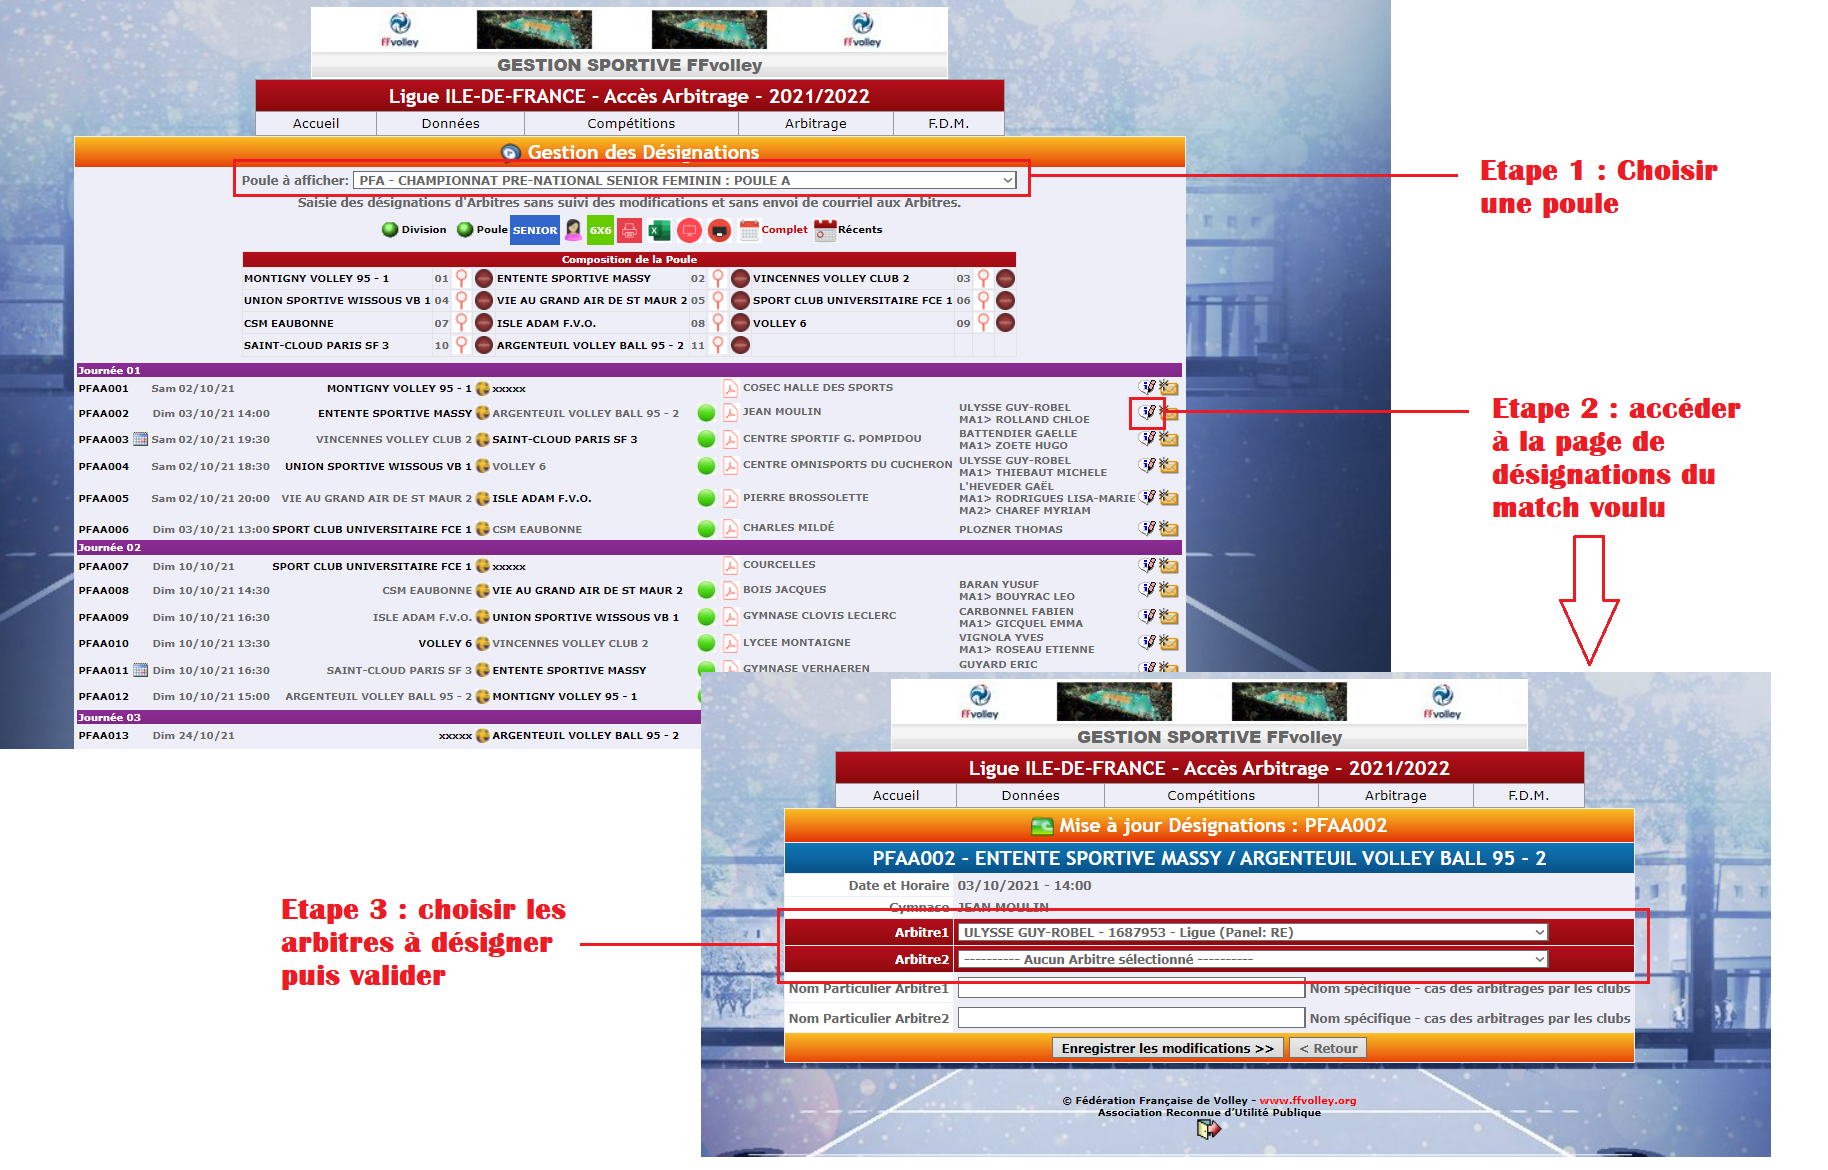
\includegraphics[width=\linewidth]{designation_avant}
    \caption{Processus de désignation des arbitres actuel}
\end{figure}

La nouvelle interface devait également servir à lancer l’algorithme d’automatisation des désignations, mais également permettre de procéder aux désignations manuellement tout en offrant le maximum d’informations possibles concernant les arbitres à désigner, le tout sur la même page. \\

Les désignations manuelles devaient pouvoir se valider de façon dynamique via AJAX, tandis que celles proposées par l’algorithme devaient pouvoir être validées via un bouton.

\begin{figure}[!h]
    \centering
    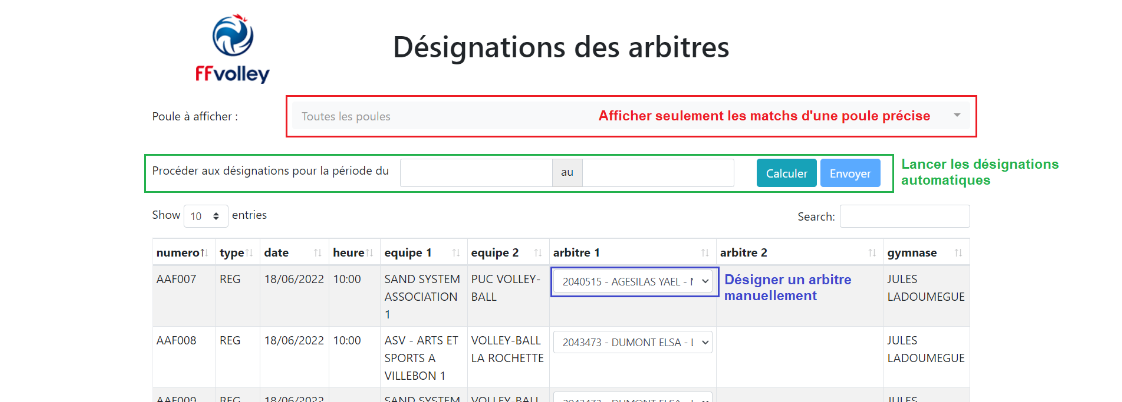
\includegraphics[width=\linewidth]{designations_mtn}
    \caption{Centralisation des informations sur la nouvelle interface}
\end{figure}

\newpage

\subsubsection{Récupération des arbitres}
\vspace{1cm}

Le calcul des disponibilités des arbitres pour chaque match étant trop long à effectuer au chargement de la page, celles-ci sont récupérées via AJAX quand l’utilisateur clique sur un SELECT.

\begin{figure}[!h]
    \centering
    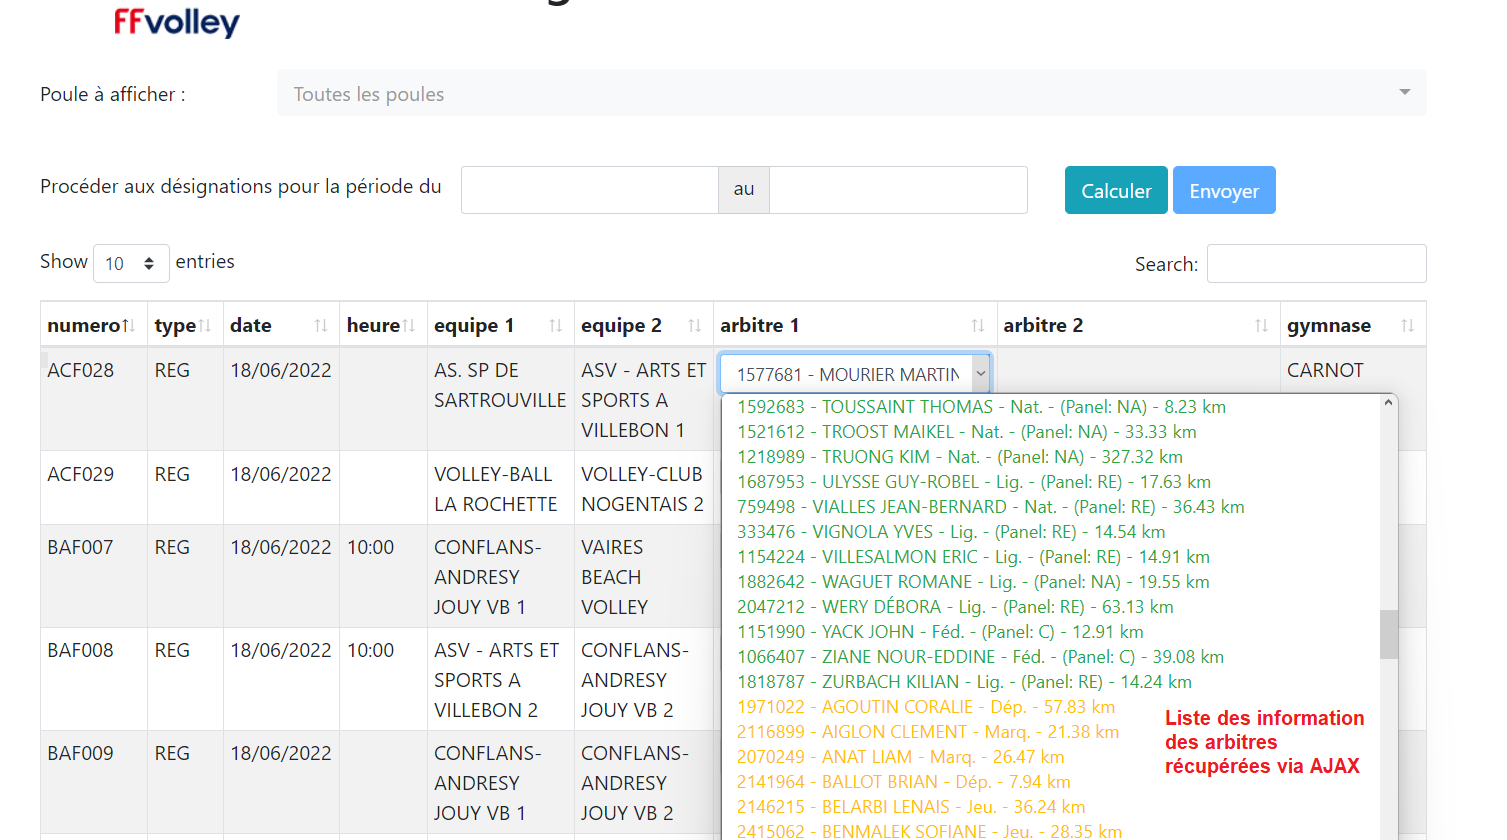
\includegraphics[width=\linewidth]{listedesg}
    \caption{Nouveau processus de désignation des arbitres}
\end{figure}

Pour faire ça, j’ai encore une fois utilisé JQuery pour envoyer une requête AJAX à une page qui récupère et me renvoi les bonnes informations d’arbitres pour le match voulu.

\begin{figure}[!h]
    \centering
    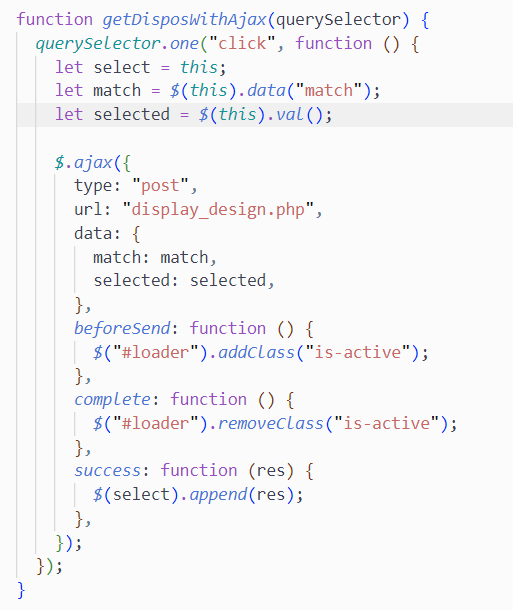
\includegraphics{getdispoajax}
    \caption{Fonction AJAX pour récupérer les arbitres}
\end{figure}

Cette façon de procéder a permis au chargement de la page de passer d’environ 180 secondes à moins de 2 secondes. Pour obtenir ces informations de performance, j’ai simplement affiché la différence en microsecondes entre la fin de mon script et le début.

\begin{figure}[!h]
    \centering
    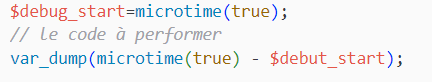
\includegraphics{debug}
\end{figure}

Au changement de sélection d’un arbitre pour le match, celui-ci est ensuite automatiquement intégré à la base de données grâce à l’envoi de ces informations via AJAX à une page annexe. Ceci permet alors d’éviter la perte de données  à un oubli.

\newpage 

\subsubsection{Désignations automatiques}
\vspace{1cm}

Pour rappel, l’algorithme de désignations automatique est construit de façon à prendre deux paramètres nullables qui correspondent aux date de la période pour laquelle effectuer ces désignations.\\ 

L’intégration de l’algorithme dans mon interface se fait donc simplement en envoyant ces valeurs via AJAX à une page annexe qui s’occupe de lancer l’algorithme et de renvoyer un tableau des matchs de la période avec les nouvelles désignations.
Ce tableau écrase ensuite celui déjà en place sur la page, et permet à son tour grâce aux fonctions Javascript de procéder aux désignations manuelles.

Les désignations automatiques doivent ensuite être validées grâce à un bouton, afin de les envoyer à une page qui s’occupe de les enregistrer dans la base de données.